\documentclass[10pt,a4paper]{article}
\usepackage[utf8]{inputenc}
\usepackage[T1]{fontenc}
\usepackage[british]{babel}
\usepackage{lmodern}
\usepackage[margin=1.8cm,top=1.6cm,bottom=1.8cm]{geometry}
\usepackage{graphicx}
\usepackage{booktabs}
\usepackage{caption}
\usepackage{float}
\usepackage{enumitem}
\usepackage[hidelinks]{hyperref}
\usepackage{xurl}

\graphicspath{{../outputs/}{../assets/}}
\captionsetup{font=small,labelfont=bf,skip=3pt}
\setlength{\parskip}{3pt}
\setlength{\parindent}{0pt}
\setlist{nosep,leftmargin=*}

\title{\vspace{-1.2cm}\textbf{Bringing Sketches to Life with Generative AI}}
\author{Nosa Peter Inwe\\[2pt]
\small Computer Vision and Machine Learning II, Université Paris-Est Créteil (UPEC)\\
\small Professor: Arezoo Ghodsifard}
\date{\small 20 November 2026}

\begin{document}
\maketitle
\vspace{-0.6cm}
\begin{center}
\small\textbf{Code repository:} \url{https://github.com/nosainwe/gen-ai-projects/tree/main/sketch-to-image-controlnet}
\end{center}

\section{Objective}

I drew a car, a house and a sword by hand and used a pretrained diffusion model to turn each drawing into a finished image. The question I study is how much of the drawn structure survives generation, and which setting controls the balance between following the sketch and producing a convincing image.

The pipeline uses Stable Diffusion 1.5~[1] with ControlNet v1.1 Scribble~[2], implemented in Python with Hugging Face Diffusers~[5]. All images in this report come from one run on a Google Colab Tesla T4 GPU.

\section{How the sketch influences the output}

\begin{figure}[H]
  \centering
  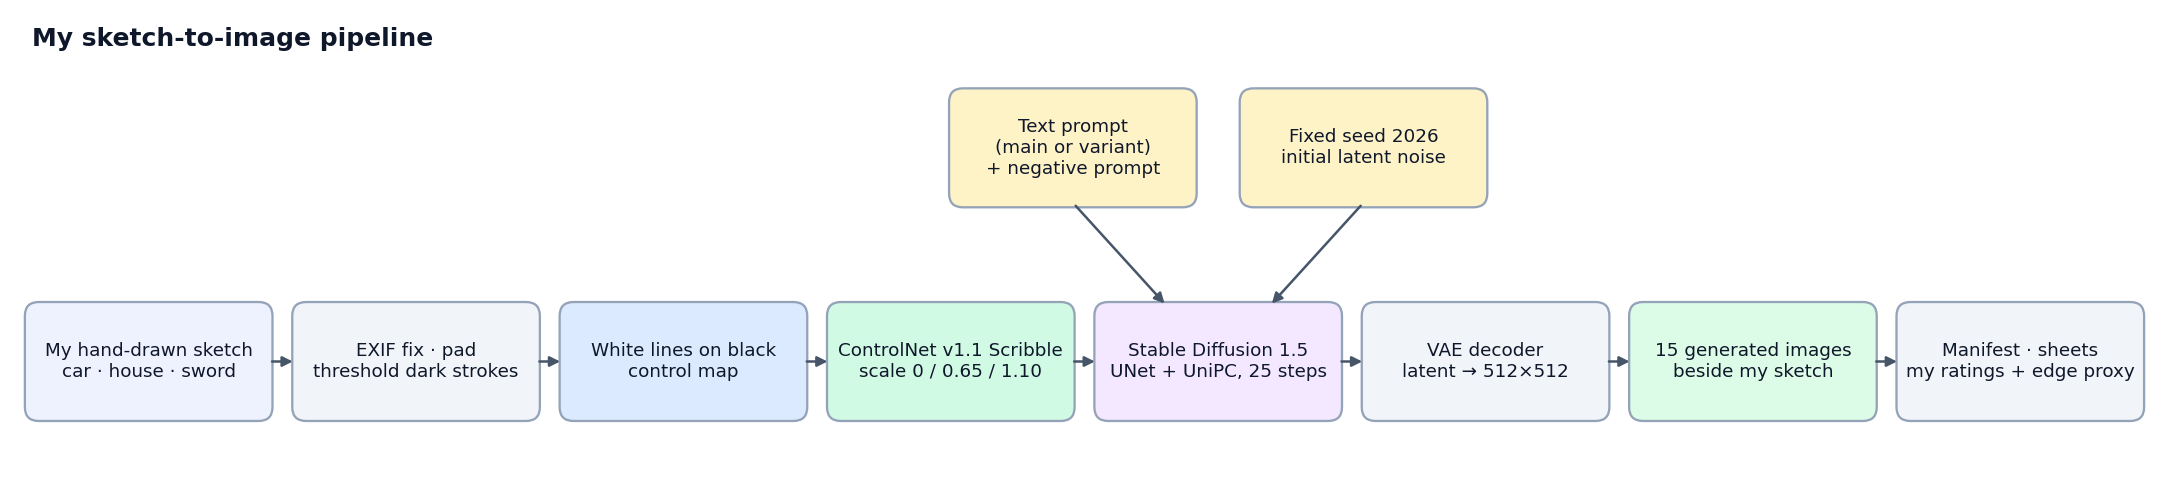
\includegraphics[width=\linewidth]{pipeline.png}
  \caption{My pipeline, from hand drawing to generated image.}
\end{figure}

\textbf{Preprocessing.} ControlNet Scribble expects white strokes on a black background. My code applies the photo's rotation flag, pads the image onto a white $512\times512$ square without stretching it, converts it to greyscale and marks every pixel darker than 205 as a stroke. I inspected the three control maps before generating; none contained shadow artefacts, so the default threshold remained unchanged.

\textbf{Stable Diffusion.} The model operates in a latent space: a variational autoencoder (VAE) compresses a $512\times512$ image into a $64\times64\times4$ latent. Generation starts from Gaussian noise in this space, and a UNet removes the noise over 25 UniPC steps~[3,4], conditioned on the prompt through the CLIP text encoder. The VAE decoder then maps the final latent back to pixels. The prompt describes the content of the image but gives no control over where objects appear.

\textbf{ControlNet.} ControlNet supplies that spatial control. It is a trainable copy of the UNet encoder that reads the control map and adds its features to the UNet at every denoising step. These connections pass through zero-initialised convolutions, so at the start of training ControlNet contributes nothing and cannot degrade the pretrained model. At inference, the parameter \texttt{controlnet\_conditioning\_scale} multiplies this contribution: a scale of 0 removes the sketch entirely, and larger values pull the image more strongly towards the strokes. Because the control map contains only lines, it determines position and outline, while the prompt determines colour and material.

\textbf{Fixed settings.} To isolate one variable per comparison, I kept the following constant: seed 2026 with a new generator for each image, guidance scale 7.0, 25 steps, $512\times512$ resolution, fp16, and the negative prompt \emph{``poor geometry, blurry, distorted, unreadable text, watermark''}.

\section{Experiments}

\begin{table}[H]
  \centering\small
  \begin{tabular}{@{}lll@{}}
    \toprule
    Experiment & Variable & Images \\
    \midrule
    1. Control strength & scale 0.00 (baseline, prompt only), 0.65 and 1.10, main prompt & 3 per sketch \\
    2. Prompt variation & two alternative prompts at scale 0.65 & 2 per sketch \\
    \bottomrule
  \end{tabular}
\end{table}

I chose 0.65 as an intermediate value and 1.10 as a value slightly above the ControlNet default of 1.0, where the sketch should dominate. The two experiments produce 15 images. I rated each image from 1 to 5 on structure (whether the silhouette and the position of its parts survive), image quality and prompt fit. I also computed an automatic edge proxy: the share of stroke pixels lying within 5 pixels of an edge in the generated image.

\section{Results}

\subsection{Experiment 1: control strength}

\begin{figure}[H]
  \centering
  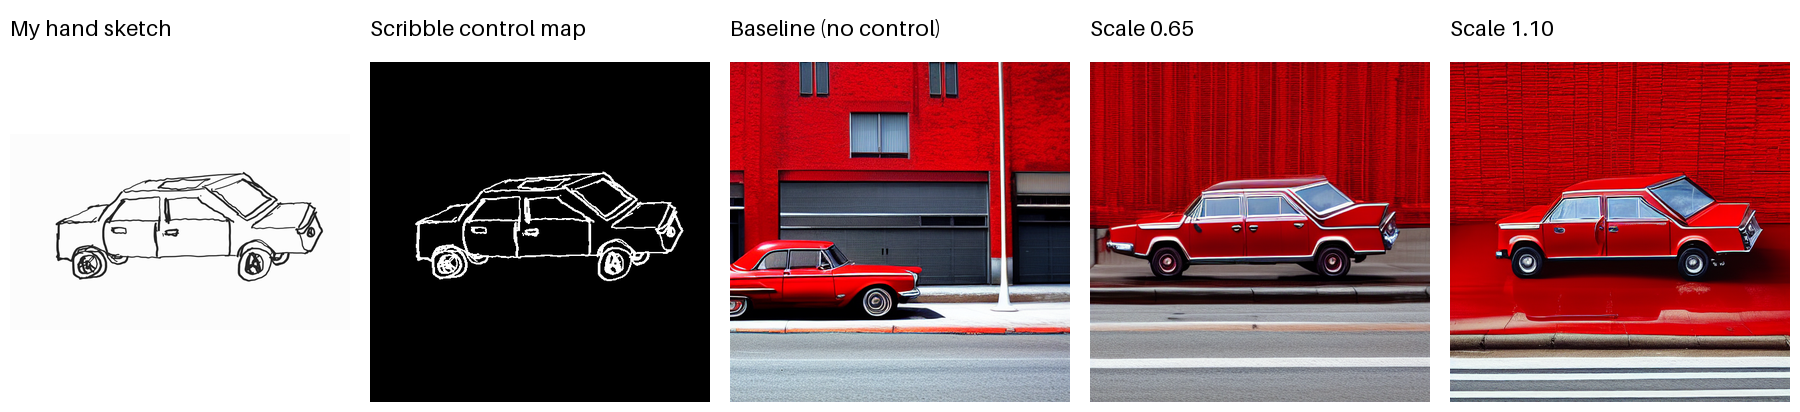
\includegraphics[width=\linewidth]{01_car_comparison.png}\\[2pt]
  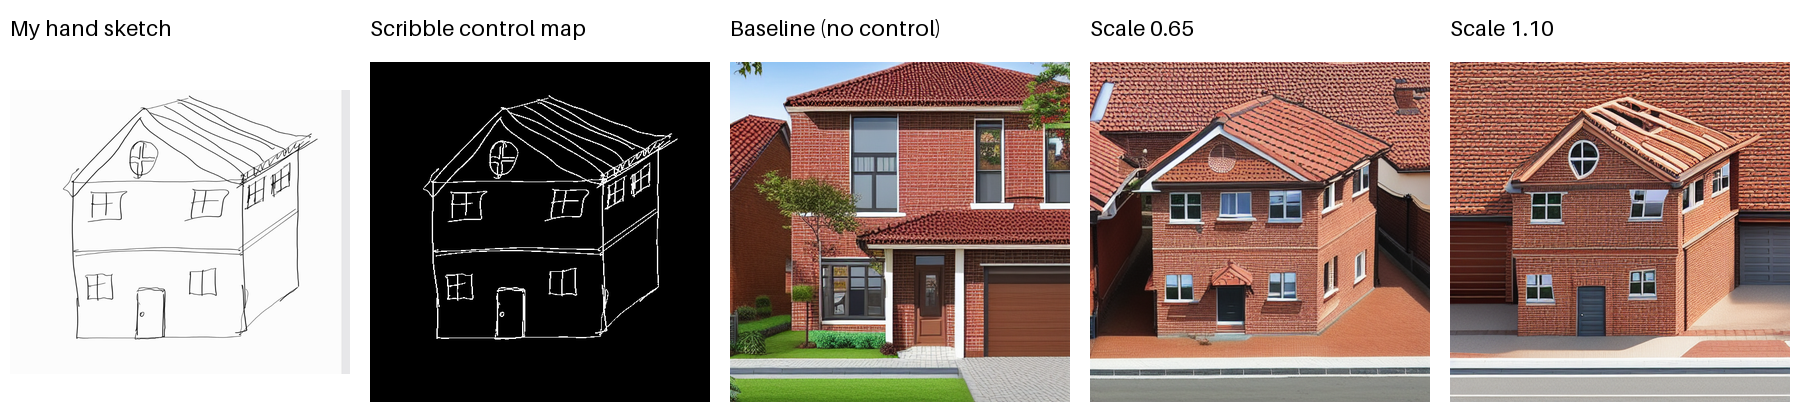
\includegraphics[width=\linewidth]{02_house_comparison.png}\\[2pt]
  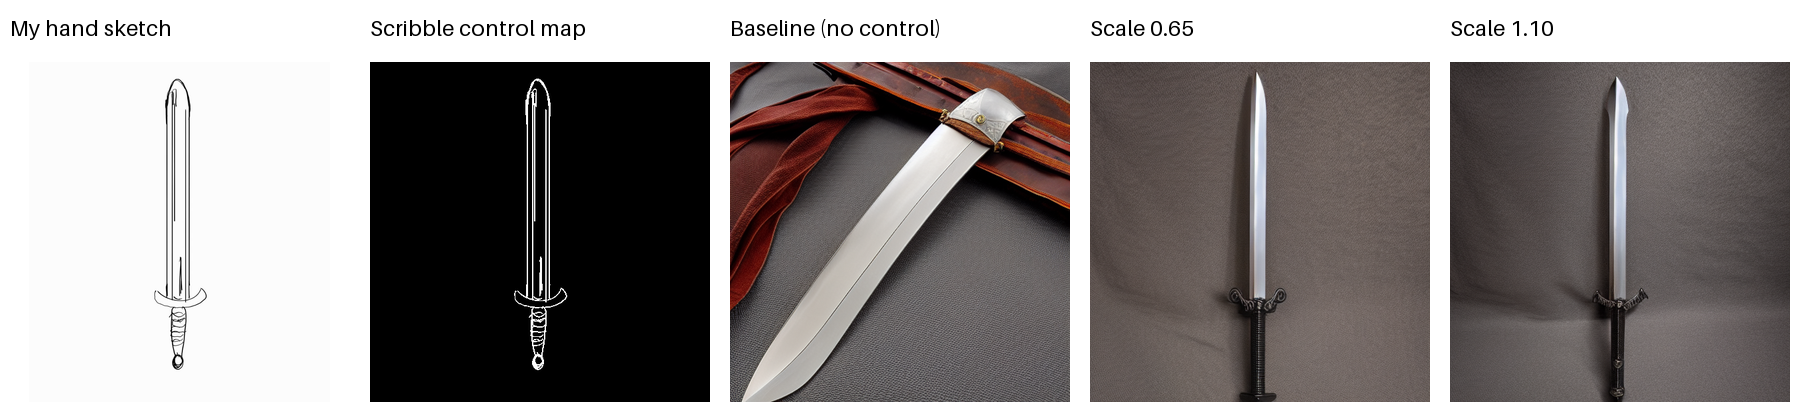
\includegraphics[width=\linewidth]{03_sword_comparison.png}
  \caption{Each row: my sketch, its control map, then scales 0.00, 0.65 and 1.10 with the main prompt.}
\end{figure}

\begin{table}[H]
  \centering\small
  \begin{tabular}{@{}ccccc@{}}
    \toprule
    Scale & Structure & Quality & Prompt fit & Edge proxy \\
    \midrule
    0.00 & 1.0 & 3.7 & 3.7 & 0.84 \\
    0.65 & 4.0 & 4.0 & 4.0 & 0.96 \\
    1.10 & 5.0 & 3.3 & 3.3 & 0.98 \\
    \bottomrule
  \end{tabular}
  \caption{Mean scores over the three sketches.}
\end{table}

At scale 0.00 the model ignores the sketch. The car is cropped at the left edge, the house becomes a frontal view with a garage, and the sword becomes a curved blade lying diagonally. These images are plausible on their own, which confirms that all structural agreement in the other images comes from ControlNet.

Scale 0.65 gives the best balance. The car keeps its side profile, door division and sloping rear window, and the model reinterprets the bulge at the rear of my drawing as tail fins. The house keeps its three-quarter view and window positions, and the sword stands upright with the crossguard and grip in the drawn positions. The main defect is colour bleeding: the phrase ``glossy red paint'' turns the background wall red as well.

At scale 1.10 the outline matches most closely, but image quality falls. The house reproduces the round attic window exactly, yet it also renders the hatching on my roof as a row of slats. The car looks like a toy, and the red colour spreads to the wall and floor. The sword is the least affected, because its outline consists mostly of straight lines.

\subsection{Experiment 2: prompt variation}

\begin{figure}[H]
  \centering
  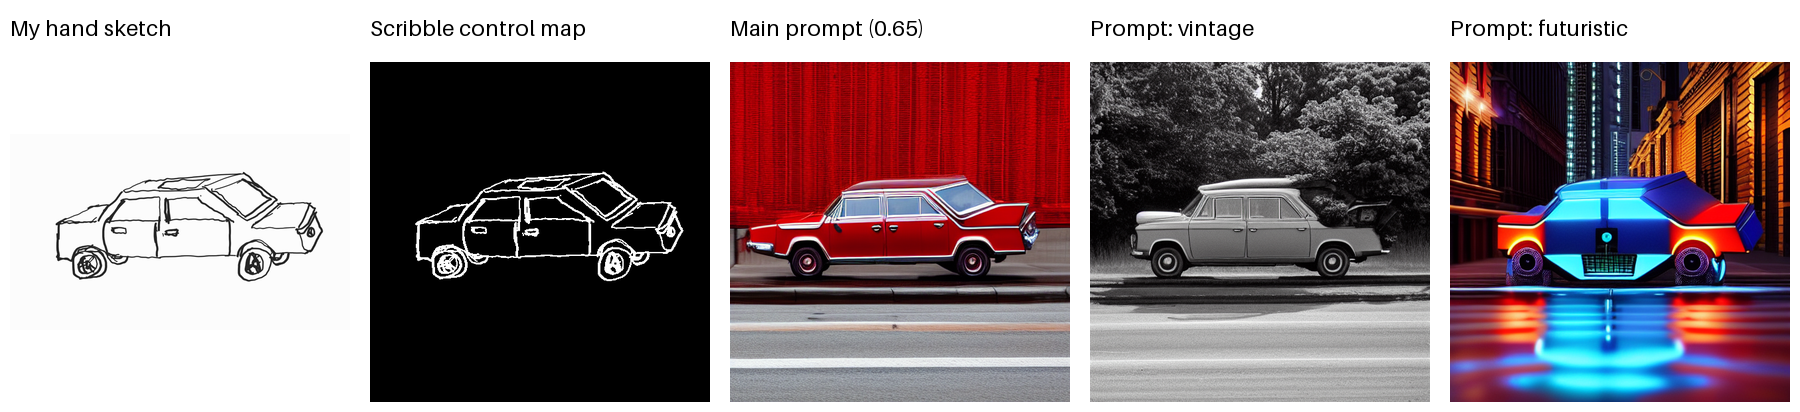
\includegraphics[width=\linewidth]{01_car_prompts.png}\\[2pt]
  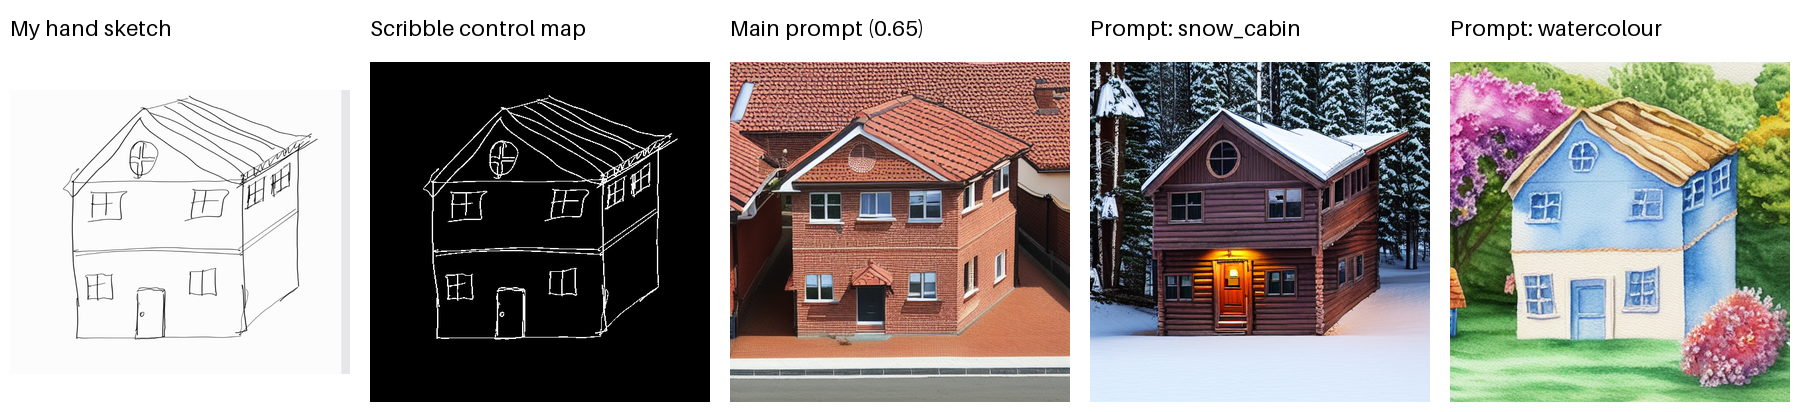
\includegraphics[width=\linewidth]{02_house_prompts.png}\\[2pt]
  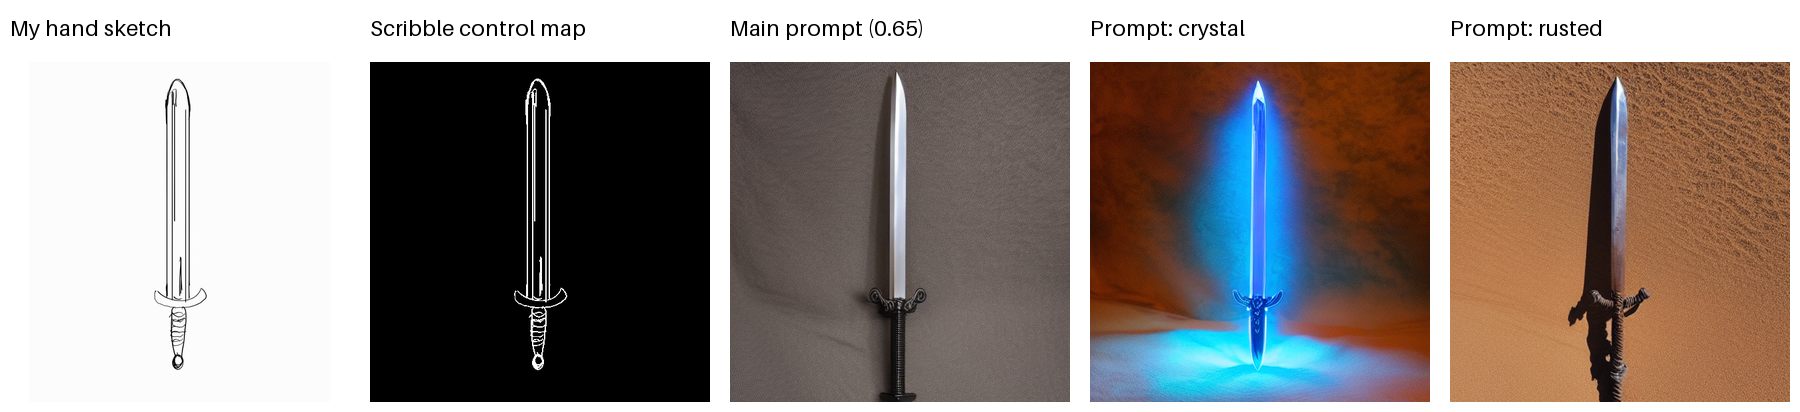
\includegraphics[width=\linewidth]{03_sword_prompts.png}
  \caption{Each row: my sketch, its control map, then the main prompt and two alternative prompts, all at scale 0.65.}
\end{figure}

The house gives the strongest results. Both the snow cabin and the watercolour cottage keep the round window and the window grid while changing material, setting and style. At this scale the sketch fixes the geometry and the prompt controls the appearance.

The car shows the limit of a moderate scale. The vintage version keeps the body and wheels, but the strokes of the rear window merge with the trees behind the car. The futuristic prompt conflicts most with the drawing: the model rebuilds the side view as a symmetric frontal body and keeps only the wheel positions. A prompt that implies a specific shape can override the sketch at 0.65.

The sword shows the opposite failure. The outline survives both prompts, but parts of the prompts do not: the crystal blade appears against an orange background instead of a dark cave, and the rusted sword still looks like clean steel.

Across the six variants, the mean structure score is 3.3, against 4.0 for the main prompts at the same scale, while prompt fit stays at 4.0. A prompt that departs further from the drawing needs a higher scale to preserve the shape.

\section{Analysis}

\textbf{The control scale is a trade-off.} Structure rises from 1.0 to 5.0 as the scale increases, while quality and prompt fit peak at 0.65 and decline at 1.10. Beyond that point, ControlNet reproduces the imperfections of a hand drawing, such as shaky lines and hatching, as part of the object. For rough sketches I would use 0.65 by default and raise it only when the prompt works against the drawn shape.

\textbf{The edge proxy does not measure sketch preservation.} It increases with the scale, from 0.84 to 0.98, but the baselines already score between 0.76 and 0.93 while ignoring the sketch. Textures such as brick, roof tiles and foliage place edges across the whole image, so many strokes fall near an edge by chance; the house baseline reaches 0.93 for this reason. My visual ratings are therefore the main evidence in this report. A stricter metric, such as matching the strokes against Canny edges of the output, would be a better choice.

\textbf{Limitations and next steps.} Each setting uses a single seed, so some differences may come from the initial noise rather than the setting. I would repeat the runs with several seeds, tune the scale per sketch, remove the roof hatching from the house drawing and replace the edge proxy with the stricter metric above.

\section{Bonus: web application}

I built a Gradio web application (\texttt{src/gradio\_app.py}) in which a user draws on a $512\times512$ canvas in the browser or uploads a photo of a sketch. Before generating, the page displays the control map and an ink check that rejects unusable photos. The prompt, scale, seed and number of steps are adjustable, and the application uses the same preprocessing and settings as the experiments. I ran it from \texttt{notebooks/02\_web\_app.ipynb} on a Colab T4 through the public Gradio link. Twelve unit tests with a mock model cover its logic.

\section{Reproducibility}

The models are \texttt{stable-diffusion-v1-5/stable-diffusion-v1-5} and \texttt{lllyasviel/control\_v11p\_sd15\_scribble} from Hugging Face (CreativeML OpenRAIL-M licence). The run used Python 3.13, PyTorch 2.14.1, Diffusers 0.39.0 and Transformers 4.57.6 on a Tesla T4; \texttt{outputs/environment.json} lists every version. To reproduce the results, open \texttt{notebooks/01\_sketch\_to\_image.ipynb} in Colab with a T4 GPU and run the cells in order, or follow the local instructions in the README. All prompts and settings are in \texttt{experiments.json}, and \texttt{outputs/run\_manifest.json} records the SHA-256 hash of each input sketch.

\section*{References}
\small
\begin{enumerate}[label={[\arabic*]}]
  \item R.~Rombach et al. High-resolution image synthesis with latent diffusion models. \emph{CVPR}, 2022. arXiv:2112.10752.
  \item L.~Zhang, A.~Rao and M.~Agrawala. Adding conditional control to text-to-image diffusion models. \emph{ICCV}, 2023. arXiv:2302.05543.
  \item J.~Ho, A.~Jain and P.~Abbeel. Denoising diffusion probabilistic models. \emph{NeurIPS}, 2020. arXiv:2006.11239.
  \item W.~Zhao et al. UniPC: a unified predictor-corrector framework for fast sampling of diffusion models. arXiv:2302.04867, 2023.
  \item Hugging Face Diffusers documentation (ControlNet pipeline) and the model cards of both models.
\end{enumerate}

\normalsize
\section*{AI assistance}
I used Claude (Anthropic) as an assistant during this project. It helped me write and test the code, the notebooks and the web application, suggested the prompts, and helped draft this report and an initial set of image scores. I drew the sketches, ran the experiments, reviewed every image and corrected the scores and analysis where they did not match my own assessment.

\end{document}
